\documentclass[a4paper]{article}

% Start Preamble
\usepackage[utf8]{inputenc}
\usepackage{fullpage}
\usepackage[english]{babel}
\usepackage{color}
\usepackage{amsmath}
\usepackage{url}
\usepackage{standalone}
\usepackage{parskip}
\usepackage[version=4]{mhchem}

\title{Lecture 2: Experimental Facts of Life}
\author{Renzo Shredder}
\date{October 4 2018}
% End Preamble

\begin{document}
\maketitle
%---------------------
\section*{Introduction}
Goal of this lecture: outline some experimental facts that we will have to deal with and should aim to understand/model as we progress throughout the course.
\\
\\
Importantly, physics doesn't tell us \textit{why} (in terms of abstract truths) the universe is the way it is. Instead, physics gives us models to help us explain how things behave and predict their behavior.
\begin{itemize}
    \item In other words, one could say the aim of physics is to develop models that give us intution for phenomena and allow us to make predictions
\end{itemize}

\section*{Facts of Life}
\begin{enumerate}
    \item Atoms exist
    \item Randomness exists 
    \item Atomic spectra: discrete, structured 
    \item Photoelectric effect 
    \item Electron diffusion
    \item Bell's Inequality 
        \begin{itemize}
            \item Note: This is in a sense, this fact is a "framework" of the course
        \end{itemize}  
\end{enumerate}

\section{Atoms Exist}
At this point, we know that a given atom is comprised of electrons and nuclei
\begin{itemize}
    \item We know electrons exist, because we (used) to see them manifest themselves in cathode ray tubes used in old TV sets 
        \begin{itemize}
            \item Aside: a \textbf{cathode ray tube} is a gun that shoots electrons at a phosphorescent screen (in the words of some famous physicist, if you can "spray" them, then they exist)
            \item Every time the electron hits the screen, it induces a phosphorescence (i.e., a "glow") onto the TV screen 
        \end{itemize}
    \item Here is a better argument for the existence of electrons: we can actually see them individually 
        \begin{itemize}
            \item One of the most famous images in physics came from an experiment called "Gargamelle" (Figure \ref{fig:gargamelle}
            \item In this experiment, a $30 \, \mathrm{m^3}$ tank of liquid freon is set so that it is pulsing (what is pulsing?) just at its vapor pressure at $60 \, \mathrm{Hz}$
            \item This experiment revealed two things:
                \begin{enumerate}
                    \item You can obtain images of individual electrons moving through fluids and leaving trails of bubbles behind them (we will talk about this later in more detail)
                    \item It is possible for a neutrino to collide with an electron; this process is called a \textbf{weak neutral current}. In other words, it proved the existence of weak neutral currents (for the purposes of this course, we wont discuss this in much detail) 
                \end{enumerate}
            \begin{figure}%
                \centering
                \label{fig:gargamelle}%
                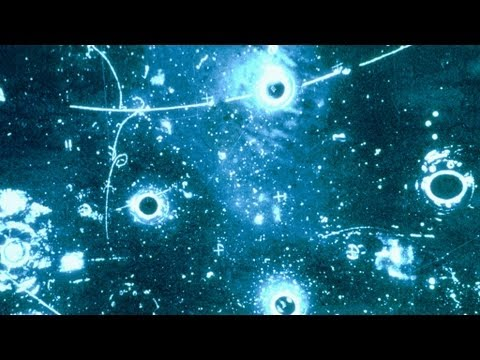
\includegraphics[height=2in]{Images/gargamelle_results.jpg}%
                \caption{Track in the Gargamelle bubble chamber at CERN from a neutrino scattering of an electron. Shows a trail of nucleated bubbles in from depressurizing freon. The path to the left-hand side that looks like an upside-down fish hook is the path of a single electron that a neutrino incident from a beam collided with}
                \label{fig:pathspacetrans}
            \end{figure}
        \end{itemize}
    \item We know nuclei exist, because you can shoot alpha particles (produced from radioactive decay - see inorganic chemistry notes) at a thin sheet of atoms
        \begin{itemize}
            \item Note: the official version of this experiment was conducted by Rutherford, Geiger, and Marsden in the late 19th century
            \item Results showed that every once and a while, these alpha particles would bounce back at near $180^\circ$ relative to its initial motion
            \item These results were surprising (analogous to a bowling ball being bounced back by a sheet of paper) 
            \item For a while, people explained this by theorizing that electrons travel along \textit{orbits} (not to be confused with the term\textit{orbital}) around high-density atomic nuclei
        \end{itemize}
    \item We also noted that we could strip (negatively charged) electrons from our sheet of atoms, and thus leaving behing the (positively charged) atomic nuclei
        \begin{itemize}
            \item Since Coulomb's law quantifies the electric force between two charged objects and it is analogous to the equation for gravity, scientists assumed the relation between electrons and nuclei followed the same laws as planets orbiting around a sun (i.e., Keplarian orbits) 
            \item First problem in the homework set will show that this logic doesn't hold
                \begin{itemize}
                    \item Recall: When you accelerate a charge, it radiates - i.e., it loses potential energy to its surroundings (heat) and kinetic energy (motion)
                    \item In other words, as our electron speeds up, its radiation increases and potential energy decreases (going to calculate how long this takes in the problem set; hint: its not very long) 
                    \item The fact that classical objects (e.g., cheese) exists tells us that our Keplarian model of electrons isn't correct
                \end{itemize}
        \end{itemize}
\end{itemize}
According to classical mechanics, electrons should not exist. But we know that they do exist... therefore classical mechanics is an "incomplete"/inaccurate description of the universe. 
\\
\\
A major goal of quantum mechanics: to concoct a model that allows for atoms to exist
\section{Randomness Exists}
Fun fact about Geiger: he later on went to invent a machine called the \textbf{Geiger counter} that detects EM radiation that our eyes cannot detect 
\begin{itemize}
    \item Aside: Increasing the potential across a capacitor past a certain threshold will produce a spark (this is how APs work!!) 
    \item For the experiment setup, Geiger isolated a capacitor in a container filled with a stable, inert gas and increased the voltage across the capacitor until he got a spark (i.e., electricity flowing across the capacitor) just enough so the equipment didn't get burned out
    \item Reasoned that passing a charge (e.g., an alpha particle - which has a +2 charge) will introduce a new electric field to our system and also induce spark "nucleation"
    \item If we set the potential across the capacitor below the "spontaneous-spark threshold potential", the presence of a spark indicates the passage of a charged particle across the capacitor 
    \item This concept is analogous to the second experiment we described during Lecture 1 (i.e., a hard electron sent through a durability box and then through a color box should output an electron that is white 50\% of the time and black 50\% of the time)  
    \begin{itemize}
        \item Similarly, with a Geiger counter, atoms decay, but they decay randomly
        \item Although we can't predict with 100\% certainly when an atom will decay, we have a pretty good idea of what the probability is that it will decay at a given point in time (Poisson process?) 
    \end{itemize}
\end{itemize}
Importantly, the Geiger counter provides a powerful argument that randomness does indeed exist. Moreover, similar experiments "hard scattering" experiments persisted throughout the 60s and 70s. And if randomness does indeed exist, it needs to be incorporated into our quantum mechanical models. 
\begin{itemize}
    \item \textbf{Hard scattering experiments} refer to experiments that send an object at very high velocities at some other object and looking for the rare events when our high-velocity object bounces off the other object at some large angle
    \item Usually, hard scattering experiments are used to detect dense cores of objects 
    \item Importantly, hard scattering experiments conducted at Stern University in the 60s and 70s showed that the proton is not a fundamental particle after shooting incident electrons at protons 
    \item Currently, we describe protons as being composit particles comprised of "three" (morally speaking anyway) point-like particles we call \textbf{quarks}
    \item Some trivial properties of quarks
    \begin{itemize}
        \item They have fractional charge (Kendall, Friedman, Taylor, et al. at MIT - they shared the nobel prize in 1990 for discovering a partonic model for the structure of nucleons) 
    \end{itemize}
\end{itemize}
An example of a current research doing hard scattering experiments involves the use of the relativistic heavy ion collider at Brookhaven
\begin{itemize}
    \item Here, we are seeing what happens when we collide two protons into each other 
    \item After the protons collide, we get a shrapnel of "proton constituents" everywhere 
    \item As it turns out, this shrapnel of proton constituents comes from a fleeting, ultra-high denisty/temperature liquid called the \textbf{RHIC fireball} that forms in areas where the protons overlap 
    \item This ball of energy is also sometimes called quark-gluon plasma... however this is misleading since the substance we are referring to is a liquid, not a plasma 
    \item Consequence of RHIC fireballs being liquid is that its \textit{dissipates} 
    \begin{itemize}
        \item Like other liquids (e.g., water), this dissipation manifests itself as physical waves 
        \item Aside: think about a cup of coffee that is cooling off. In order to warm it up again, we can add in some hot coffee. When we first add the hot coffee, the system is out of equilibrium. However, over some time, the coffee will return to thermal equilibrium. Q: How long does it take for the coffee to come to equilibrium? 
        \begin{itemize}
            \item More specifically, how long does it take your coffee to reach equilibrium relative to how long it takes for a photon to travel across your mug?
            \item A: the time it takes for the coffee to return to thermal equilibrium is magnitudes slower than the time it takes for the photon to travel across the mug. 
        \end{itemize}
        \item In the case of our RHIC fireball liquid, the time it takes for our shrapnel of proton constituents from the RHIC fireball to return to a state of thermal equilibrium is proportional to the time it takes for a photon to travel across our liquid "puddle" of RHIC fireball
        \item Note: liquids such as the RHIC fireball that behave this way are called \textbf{quantum liquids}
    \item Fun fact: A good model for describing quantum liquids is that used to describe black holes 
    \end{itemize}
\end{itemize}
\section{Atomic Spectra: Discrete, Structured}
Lets consider an experiment like to the one described by the Geiger counter using some given inert gas and consider the following sequence of events:
\begin{itemize}
    \item Any time a spark is produced, we can conclude some of our gas molecules were excited for a few fleeting moments and will consequently emit light
    \item Say put a prism in the path of the light emitted from the excited gas molecules 
    \item If we look at an image of the light emitted after it has passed through the prism, we will see a set of DISCRETE and DISTINCT colored bands 
\end{itemize}
The \textbf{Rydenberg} constant can be used to explain the entire spectra of spectral lines for Hydrogen gas through the following formula: 
\begin{equation}
    \frac{1}{\lambda} = R \left( \frac{1}{m^2} - \frac{1}{n^2} \right), \quad n>m
\end{equation}
Moreover, for every other element, there exists some equation such as this that perfectly predicts its corresponding spectral lines 
\begin{itemize}
    \item Our quantum mechanical model of the world needs to explain this phenomena 
\end{itemize}
\section{Photoelectric Effect}
Shining light on a metal beam can cause electrons to bounce off the beam
\begin{itemize}
    \item Aside: research that investigates the interaction between light and piece of metal are done in condensed matter labs
    \item Things they measure: the kinetic energy and number of the electrons that are emitted as a function of the intensity of light that is shown on the metal beam
    \item Experimental setup for measuring the kinetic energy of an electron that is been excited through this \textbf{photoelectric effect}
\end{itemize}
\subsection*{Goal of the Experiment}
For a given a beam of electromagnetic radiation with energy (which is proportional to intensity) $E_\gamma$ and frequency $\nu$, find the threshold voltage $V_0=E_0/q$ for which the current passing through the circuit is $I=0 \mathrm{A}$.
\subsection*{Independent variables}
\begin{enumerate}
    \item Light intensity $I \propto \vec{E}^2 + \vec{B}^2 \quad [\mathrm{W/m^2}] = [\mathrm{(J/s)/m^2}]=[\mathrm{(1/s)(J/m^2)}]$
    \item Light frequency $\nu \quad [\mathrm{1/s}]$
\end{enumerate}
\subsection*{Expected Results} 
\begin{enumerate}
    \item As we increase the intensity (i.e., energy) of the light beam, the kinetic energy that is  transfered to the emitted electrons should increase, thus increasing the magnitude of the threshold potential. 
    \begin{itemize}
        \item These predictions are based off Maxwellian dynamics 
        \item Recall: the energy associated with an electromagnetic way can be modeled as a harmonic oscillator 
        \item This is a consequence of the frequency associated with the EM wave "canceling out" such that the energy associated with any given electromagnetic wave equals the amplitude of the harmonic function modeling the wave
    \end{itemize}
    \item The threshold voltage should be independent of the frequency of the light beam. 
\end{enumerate}

\subsection*{Actual Results}
\subsection*{Planck's Constant Background}
The idea that the energy of an electromagnetic wave benig linearly propertional to its frequency first came from the analysis of blackbody radiation by a guy named Planck. 
\begin{itemize}
    \item Planck tried to show $E_{\gamma}=h\nu$ via fitting $h$ with an experimental curve (Note: adults shouldn't be curve fitting - and he hated doing it) 
    \item He had a theory predicting the amount of energy emitted by an object that was hot and glowing as a function of frequency. This theory turned out to completely disagree with experiments unless he set $h=6.626\cdot 10^{-34} \quad \mathrm{J/s}$ 
    \item This combined with Einstein's 1905 paper ended up revolutionizing physics since it implied that light behaves as a particle (Einsteind ended up getting the Nobel prize for this) 
\end{itemize}
Note: for the past 200 years, mainstream physics had become convinced that light only behaves as a wave (double-slit experiment) 
\section{Electron Diffusion}
\subsection*{Bucky  Ball Experiment}
Question: do bucky balls interfere with themselves? 
\begin{itemize}
    \item Want to redo a electric diffusion experiment with bucky balls (\ce{C_{60}})
    \itme However, quantum effects for macroscopic objects are usually insignificantly small
    \item Note: in principle, we should be able to generalize our results to other macroscopic objects 
    \item Experiment description
    \begin{itemize}
        \item Heat up the bucky balls in an oven and emit them with some definite thermal energy 
        \item Then we columntate then by sending them through a single slit 
        \item Then, the bucky balls pass through a diffraction grating and are imaged using photo ionization to see their horizontal position 
        \item Two different conditions:
        \begin{enumerate}
            \item Without grating we get a normally distributed peak of samples that land in the middle of the "landing" screen
            \item With grating, we still get a peak in the middle of the "landing" screen, but on each side of the peak, there are interference fringes 
        \end{enumerate}
        \item Conclusion: we have macroscopic objects interfereing with themselves, even as we shoot them out of the electron beam one-by-one
    \end{itemize}
\end{itemize}
\section{Bell's Inequality}
Consider the following scenario:
\begin{itemize}
    \item Variables:
    \begin{itemize}
        \item $\mathrm{Num}(U)=$ number of undergraduates in the class
        \item $\mathrm{Num}(\Bar{U})=$ number of graduates in the class
        \item $\mathrm{Num}(B)=$ number of blondes in the class
        \item $\mathrm{Num}(\Bar{B})=$ number of non-blondes in the class
        \uten $\mathrm{Num}(M)=$ number of people from Massachusetts in the class
        \item $\mathrm{Num}(\Bar{M})=$ number of people not from Maryland in the class
    \end{itemize}
    \item Say we claim the following inequality: 
        \begin{equation}
            \mathrm{Num}(U,\Bar{B}) + \mathrm{Num}(B,\Bar{M}) \geq \mathrm{Num}(U,\Bar{M})
        \end{equation}
    \item e.g., for the actual class in the lecture
        \begin{itemize}
            \item $\mathrm{Num}(U,\Bar{B})=14$
            \item $\mathrm{Num}(B,\Bar{M})=1$
            \item $\mathrm{Num}(U,\Bar{M})=15$ 
                \begin{itemize}
                    \item The samples from the class satisfy the inequality condition 
                \end{itemize}
        \end{itemize}
 \end{itemize}   
Proof for the inequality:
\begin{itemize}
    \item $\mathrm{Num}(U,\Bar{B})$ also can be thought of as the number of people in the class who are undergraduates, not blonde and from Massachusetts plus the number of people who are undergraduates, not blonde and not from Massachusetts:
        \begin{equation}
            \mathrm{Num}(U,\Bar{B}) = \mathrm{Num}(U,\Bar{B},M) + \mathrm{Num}(U,\Bar{B},\Bar{M})
        \end{equation}
    \item $\mathrm{Num}(B,\Bar{M})$ also can be thought of as the number of people in the class who are blonde, not from Massachusetts, and undergraduates plus the number of people who are blonde, not from Massachusetts, graduates:
        \begin{equation}
            \mathrm{Num}(B,\Bar{M}) = \mathrm{Num}(B,\Bar{M},U) + \mathrm{Num}(B,\Bar{M},\Bar{U})
        \end{equation}
    \item $\mathrm{Num}(U,\Bar{M})$ also can be thought of as the number of people in the class who are undergraduates,not from Massachusetts, and blonde plus the number of people who are undergraduates, not from Massachusetts, and not blonde:
        \begin{equation}
            \mathrm{Num}(U,\Bar{M}) = \mathrm{Num}(U,\Bar{M},B) + \mathrm{Num}(U,\Bar{M},\Bar{B})
        \end{equation}
    \item Lets rewrite our equation using the equalities defined above: 
    \begin{equation}
        \left(\mathrm{Num}(U,\Bar{B},M) + \mathrm{Num}(U,\Bar{B},\Bar{M})\right) + \left(\mathrm{Num}(B,\Bar{M},U) + \mathrm{Num}(B,\Bar{M},\Bar{U})\right) \geq \mathrm{Num}\left(U,\Bar{M},B) + \mathrm{Num}(U,\Bar{M},\Bar{B}\right)
    \end{equation}
    \item Simplifying gives us the following inequality:
    \begin{equation}
        \mathrm{Num}(U,\Bar{B},M) + \mathrm{Num}(B,\Bar{M},\Bar{U}) \geq 0
    \end{equation}
    \item Our end result makes sense since it implies you cant have a negative number of people in a room (which agrees with reality as we know it)
\end{itemize}
General conclusions: the number of elements in a set where each element in that set has a binary properties $A$, $B$, and $C$ satisfies the following inequality
\begin{equation}
    \mathrm{Num}(A,\Bar{B}) + \mathrm{Num}(B,\Bar{C}) \geq \mathrm{Num}(A,\Bar{C})
\end{equation}
Importantly, this inequality is called \textbf{Bell's inequality}.
\begin{itemize}
    \item Here, we were able to derive this inequlaity using logic and integers! 
\end{itemize}
Conundrum: Electrons have a third property in addition to "color" and "hardness": "whimsyness" where the electron can be whimsical or not whimsical. Let's define the various possible states of an electron as follows:
\begin{itemize}
    \item $H=$ hard and $\Bar{H}=$ soft
    \item $C=$ black and $\Bar{C}=$ white
    \item $W=$ whimsical and $\Bar{W}=$ not whimsical
\end{itemize}
Now, say we perform an experiment on a set of electrons where we measure the following: 
\begin{itemize}
    \item The number of electrons that are hard and not black, $\mathrm{Num}(H,\Bar{C})$
    \item The number of electrons that are black and not whimsical, $\mathrm{Num}(C,\Bar{W})$
    \item The number of electrons that are hard and not whimsical, $\mathrm{Num}(H,\Bar{W})$
\end{itemize}
Aside: Let's prime ourselves for interpreting our three arbitrary binary properties of electrons by redefining each variable as follows: 
\begin{itemize}
    \item Hardness corresponds with angular momentum along the $x$-axis
        \begin{itemize}
            \item $H$ corresponds with positive angular momentum along the $x$ axis and is denoted $\uparrow_x$
            \item $\Bar{H}$ corresponds with negative angular momentum along the $x$ axis and is denoted $\downarrow_x$
        \end{itemize}
    \item Color corresponds with angular momentum along the $y$-axis
        \begin{itemize}
            \item $C$ corresponds with positive angular momentum along the $y$ axis and is denoted $\uparrow_y$
            \item $\Bar{C}$ corresponds with negative angular momentum along the $y$ axis and is denoted $\downarrow_y$
        \end{itemize}
    \item Whimsyness corresponds with the angular momentum along the $z$-axis
        \begin{itemize}
            \item $W$ corresponds with positive angular momentum along the $z$ axis and is denoted $\uparrow_z$
            \item $\Bar{W}$ corresponds with negative angular momentum along the $z$ axis and is denoted $\downarrow_z$
        \end{itemize}
\end{itemize}
Importantly, if we perform this experiment and measure our three variables for each electron, we end up with the following inequality:
\begin{equation}
    \mathrm{Num}(H,\Bar{C}) + \mathrm{Num}(C,\Bar{W}) < \mathrm{Num}(H,\Bar{W})
\end{equation}
Formally, this translates to...
\begin{equation}
    \mathrm{Num}(\uparrow_x,\downarrow_y) + \mathrm{Num}(\uparrow_y,\downarrow_z) < \mathrm{Num}(\uparrow_x,\downarrow_z)
\end{equation}
Another way we can write this equation is as follows:
\begin{equation}
    \mathrm{Num}(\uparrow_0,\downarrow_{\theta}) + \mathrm{Num}(\uparrow_{\theta},\downarrow_{2\theta}) < \mathrm{Num}(\uparrow_0,\downarrow_{2\theta})
\end{equation}
Although we haven't reached a point where we can explain the actual meanings of each variable in the above equation, we should be deeply troubled by these results. Note that we are still assuming these three arbitrary properties are binary. Thus, a mathematical statement we derived from a purely logical perspective turns out to be false (and not just in quantum mechanics!). In fact, later we will use predictive quantum mechanics to show that Bells inequality is violated for all reality.  
\\
\\
Next lecture: going to discuss how our classical approach towards logic, integers, and adding probabilities is misguided. Then we will find a new method for adding probabilities that involves quantum mechanics. 
\end{document}

